% $Header: /cvsroot/latex-beamer/latex-beamer/solutions/generic-talks/generic-ornate-15min-45min.en.tex,v 1.5 2007/01/28 20:48:23 tantau Exp $

\documentclass{beamer}

\usetheme{Madrid}
\usecolortheme{beaver}
\usepackage{graphicx} % Allows including images
\usepackage{booktabs} % Allows the use of \toprule, \midrule and \bottomrule in tables
\usepackage{xcolor}


\usepackage[absolute,overlay]{textpos}
\usepackage{tikz}
\usepackage{pgfgantt}
\usetikzlibrary{backgrounds}

% This file is a solution template for:

% - Giving a talk on some subject.
% - The talk is between 15min and 45min long.
% - Style is ornate.

 \newcommand<>{\PutAt}[3][0pt]{%
    {\only#4{\begin{textblock*}{#1}#2%
      #3
    \end{textblock*}}}%
  }



\newcommand<>{\NormalBox}[2][]{%
  \only#3{\tikz[#1, every node/.style={shape=rectangle,draw,fill=white, #1}]\node []{#2};}
}

\definecolor{olive}{rgb}{0.3, 0.4, .1}
\definecolor{fore}{RGB}{249,242,215}
\definecolor{back}{RGB}{51,51,51}
\definecolor{title}{RGB}{255,0,90}
\definecolor{dgreen}{rgb}{0.,0.6,0.}
\definecolor{gold}{rgb}{1.,0.84,0.}
\definecolor{JungleGreen}{cmyk}{0.99,0,0.52,0}
\definecolor{BlueGreen}{cmyk}{0.85,0,0.33,0}
\definecolor{RawSienna}{cmyk}{0,0.72,1,0.45}
\definecolor{Magenta}{cmyk}{0,1,0,0}



\newtheorem{algorithm}{Algorithm}


\newcommand*\oldmacro{}%
\let\oldmacro\insertshorttitle%
\renewcommand*\insertshorttitle{%
  \oldmacro\hfill%
  \insertframenumber\,/\,\inserttotalframenumber}

\usepackage[english]{babel}
% or whatever

\usepackage[latin1]{inputenc}
% or whatever

\usepackage{times}
\usepackage[T1]{fontenc}
% Or whatever. Note that the encoding and the font should match. If T1
% does not look nice, try deleting the line with the fontenc.


\title[]{Machine Learning in Safety-Critical Domain} % The short title appears at the bottom of every slide, the full title is only on the title page

%\subtitle
\author[]{Arvind Easwaran}
\institute[NTU]{ Nanyang Technological University, Singapore}



\date[08/07/2015]{July 8, 2015}



\pgfdeclareimage[height=0.7cm]{university-logo}{logo.png}
\logo{\pgfuseimage{university-logo}}



% Delete this, if you do not want the table of contents to pop up at
% the beginning of each subsection:
\AtBeginSection[]
{
  \begin{frame}<beamer>{Outline}
    \tableofcontents[currentsection]
 \end{frame}
}


% If you wish to uncover everything in a step-wise fashion, uncomment
% the following command: 

% \beamerdefaultoverlayspecification{<+->}

% \setbeameroption{show notes on second screen=left}

\begin{document}

\begin{frame}
  \titlepage
\end{frame}

% \begin{frame}{Outline}
  % \tableofcontents
  % You might wish to add the option [pausesections]
% \end{frame}

% \section{System Model \& Motivation}




\begin{frame}[t]{Machine Learning  Application in Safety Critical Environments}
\begin{columns}[T] % align columns
\begin{column}[t]{.52\textwidth}
\color{red}\rule{\linewidth}{2pt}
\vspace{-5mm}
\begin{itemize}
\visible<1,2,3>{
  \item Decision making in life-threatening conditions (diagnosis, prognosis,machine learning-based medical decision support systems).}
  \visible<2,3>{
  \item  Robots (surgical robots, industrial robots, etc)}
  \visible<3>{
    \item  Autonomous vehicles.

\begin{figure}[h]
\centering
\caption{Autonomous Bus}
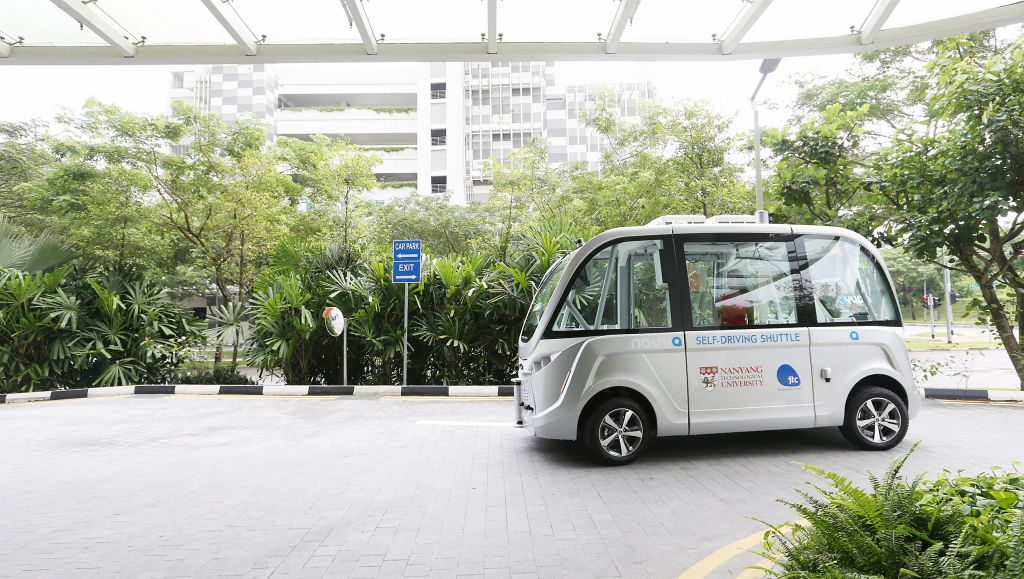
\includegraphics[scale=0.07]{fig/car.jpeg} 
\end{figure}
}
\end{itemize}

\end{column}%
\hfill%


\begin{column}[t]{.44\textwidth}
\color{blue}\rule{\linewidth}{2pt}
\vspace{-10mm}
\visible<1,2,3>{
\begin{figure}[h]
\centering
\caption{Machine Learning Based Brain Disease Diagnosis$^1$}
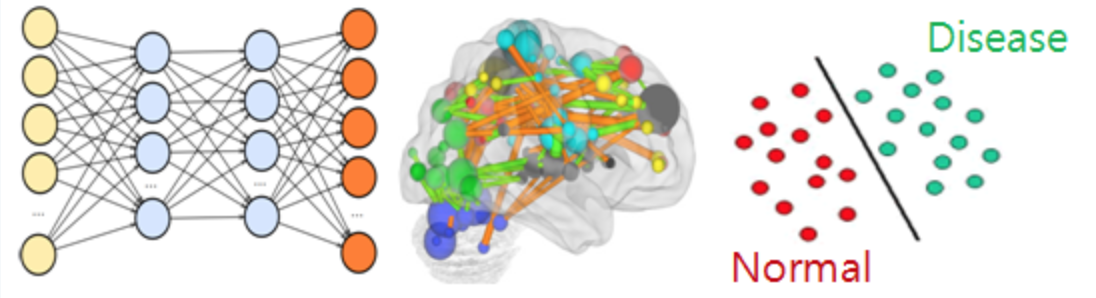
\includegraphics[scale=0.2]{fig/medical.png} 
\end{figure}
}

\visible<2,3>{
 \begin{figure}[h]
\centering
\caption{Surgical Robots$^2$}
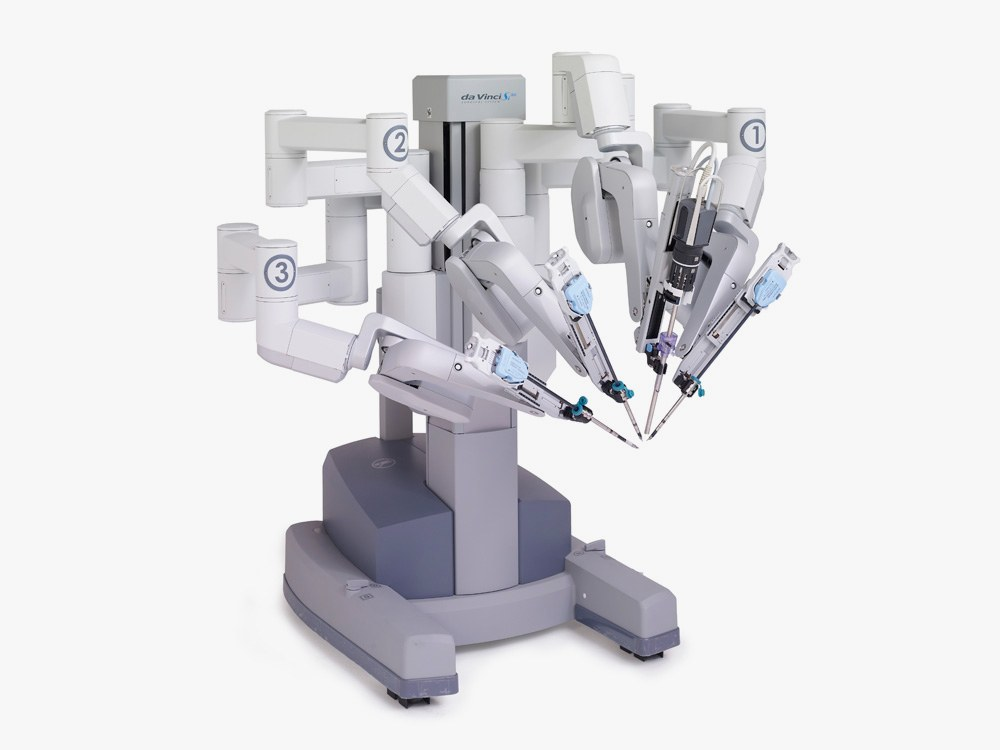
\includegraphics[scale=0.08]{fig/surgical.jpg} 
\end{figure}
}




\end{column}%
\end{columns}

  
\end{frame}



\begin{frame}[t]{Challenges to Achieve Safety}

\setbeamercovered{transparent}
\begin{itemize}
\visible<1,2,3,4>{
  \item  \textcolor{blue}{Non-transparency}: It is difficult to assess the reliability if  the reasoning behind  these models could not be understood.
  }
  \visible<2,3,4>{
  \item  \textcolor{blue}{Error Rate}:The estimate of error rate of a ML model with respect to the test data is not reliable.
  }
  \visible<3,4>{
  \item     \textcolor{blue}{Instability} A small change in the training process may produce a different result, and hence it is difficult to debug models or reuse parts of previous safety assessments.
  }
  \visible<4>{
  \item \textcolor{blue}{Difficulty in verification}: Formal verification of machine learning components is a difficult, and somewhat ill-posed problem due to the complexity of the underlying machine learning algorithms, large feature spaces.
}
\end{itemize}

\end{frame}



\begin{frame}[t]{Potential Strategies for Achieving Safety}
\begin{columns}[T] % align columns
\begin{column}[t]{.52\textwidth}
\color{red}\rule{\linewidth}{2pt}
\vspace{-5mm}
\begin{itemize}
\visible<1,2,3>{
  \item  \textcolor{blue}{Interpretability \& Transparency}: Improve the  interpretability \& transparency of the ML component.}
  \visible<2,3>{
  \item   \textcolor{blue}{Safe Fail}: The model reports that it cannot reliably give a prediction and does not attempt to do so, thereby failing safely. 
  }
  \visible<3>{
    \item \textcolor{blue}{Abstract}.  Abstract the ML component and  input  feature space  and identify scenarios that could cause violation of safety specification.
}
\end{itemize}

\end{column}%
\hfill%


\begin{column}[t]{.44\textwidth}
\color{blue}\rule{\linewidth}{2pt}
\vspace{-10mm}
\visible<1,2,3>{
\begin{figure}[h]
\centering
\caption{Explanations make the user to trust the prediction~\cite{lime}}
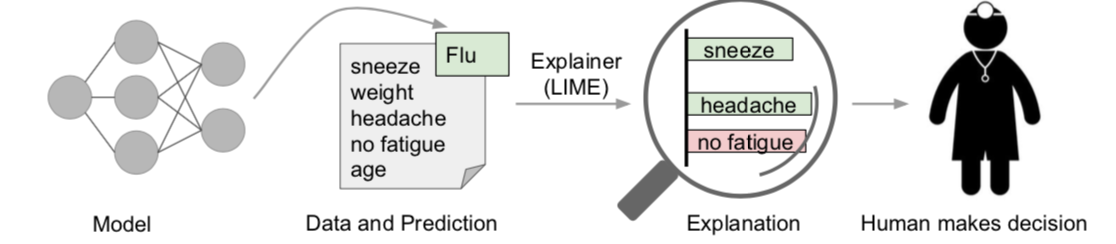
\includegraphics[scale=0.25]{fig/lime.png} 
\end{figure}
}


\visible<2,3>{
\color{black}
A technique used in machine learning when predictions cannot be given confidently is the {\color{red} reject option}~\cite{reject}.

\begin{small}
  \begin{align*}
  \hat y(x)=\begin{cases}-1~\mbox{ if  }\phi(x)\leq t\\\mbox{reject, if }\phi( x)\in(-t,t)\\1~\mbox{ if  }\phi(x)\geq t\end{cases}
\end{align*}
\end{small}


}




\end{column}%
\end{columns}

  
\end{frame}





\renewcommand{\refname}{~}
\begin{thebibliography}{1}

\bibitem{}http://mlcenter.postech.ac.kr/healthcare


\bibitem{}https://www.wired.com/2015/03/google-robot-surgery/

\bibitem{lime} Ribeiro, Marco Tulio, Sameer Singh, and Carlos Guestrin. "Why should i trust you?: Explaining the predictions of any classifier." Proceedings of the 22nd ACM SIGKDD International Conference on Knowledge Discovery and Data Mining. ACM, 2016.

\bibitem{reject} Bartlett P L, Wegkamp M H. Classification with a reject option using a hinge loss[J]. Journal of Machine Learning Research, 2008, 9(Aug): 1823-1840.

\end{thebibliography}

\end{document}